% This is my HW 8 solution set.

\documentclass[12pt, leqno]{article}
\usepackage{amsfonts, amsmath, amssymb}
\usepackage{amsbsy}
\usepackage{fancyhdr}
\usepackage{hyperref}
\usepackage{graphicx}
\newcounter{qcounter}
%\usepackage[landscape]{geometry}% http://ctan.org/pkg/geometry
%\usepackage{array}% http://ctan.org/pkg/array
\usepackage[lofdepth,lotdepth]{subfig}
\usepackage[maxfloats=40]{morefloats}
\usepackage{float}
\usepackage{}
\usepackage[english]{babel}
\usepackage{tabularx}
\usepackage{scalerel}
\providecommand{\abs}[1]{\lvert#1\rvert} % absolute value
\providecommand{\normd}{\mathcal{N}} % normal distribution
\providecommand{\norm}[1]{\lVert#1\rVert} % norm
\usepackage{mathtools}
\DeclarePairedDelimiter\ceil{\lceil}{\rceil}
\DeclarePairedDelimiter\floor{\lfloor}{\rfloor}
\newcommand{\macheps}{\epsilon_{\mbox{\scriptsize mach}}}
\usepackage[ampersand]{easylist}
\makeatletter
\newcommand{\distas}[1]{\mathbin{\overset{#1}{\kern\z@\sim}}}%
\newsavebox{\mybox}\newsavebox{\mysim}
\newcommand{\distras}[1]{%
  \savebox{\mybox}{\hbox{\kern3pt$\scriptstyle#1$\kern3pt}}%
  \savebox{\mysim}{\hbox{$\sim$}}%
  \mathbin{\overset{#1}{\kern\z@\resizebox{\wd\mybox}{\ht\mysim}{$\sim$}}}%
}
\makeatother
%\usepackage{pdflscape}


\begin{document}
\pagestyle{fancy}
\lhead{Syed Rahman}
\rhead{CIS6930}

\begin{center}
{\large {\bf Homework 1}} \\
\end{center}

\paragraph{1}
Note that 
$$
\norm{x-y}^2 = <x-y,x-y> = <x,x> - 2<y,x> + <y,y>
$$
 Similary, 
$$
\int_0^1(x(t)-y(t))^2 dt = \int_0^1 x(t)^2 dt - 2 \int_0^1 x(t)y(t) dt + \int_0^1 y(t)^2 dt
$$
Hence, we can deduce that inner product that induces the above norm is 
$$
<x,y> = \int_0^1 x(t)y(t) dt
$$
Thus to get the coefficients for the basis $B = \{1,t,t^2\}$ we need to solve the system 
$$
Ga = x
$$
for $a$, where $G_{ij} = \int_0^1B_iB_j dt$ and $x_i = \int_0^1 e^t B_i dt $. 

In $\mathbf{R}$, the following lines of code solves this system for us:
\begin{verbatim}
A[1,1] = integrate(function(t){rep(1,length(t))}, 0, 1)$value
A[2,1] = A[1,2] = integrate(function(t){t}, 0, 1)$value
A[3,1] = A[1,3] = integrate(function(t){(t^2)}, 0, 1)$value
A[3,2] = A[2,3] = integrate(function(t){(t^3)}, 0, 1)$value
A[2,2] = integrate(function(t){(t^2)}, 0, 1)$value
A[3,3] = integrate(function(t){(t^4)}, 0, 1)$value

b <- matrix(0,nrow = 3, ncol = 1)
b[1] = integrate(function(t){(exp(t))}, 0, 1)$value
b[2] = integrate(function(t){(exp(t))*t}, 0, 1)$value
b[3] = integrate(function(t){(exp(t))*(t^2)}, 0, 1)$value

a = solve(A,b)
\end{verbatim}

Figure \ref{fig:hw1p1} shows us a comparison of how the method described above is superior to the Taylor expansion in estimating $e^t$ for $t \in [0,1]$. To further support this, we also find that $\norm{x-\hat{x}} = 2.783544e^{-05}$ whereas $\norm{x-x_{Taylor}} = 0.006349231$.

\begin{figure}[H]
\begin{center}
  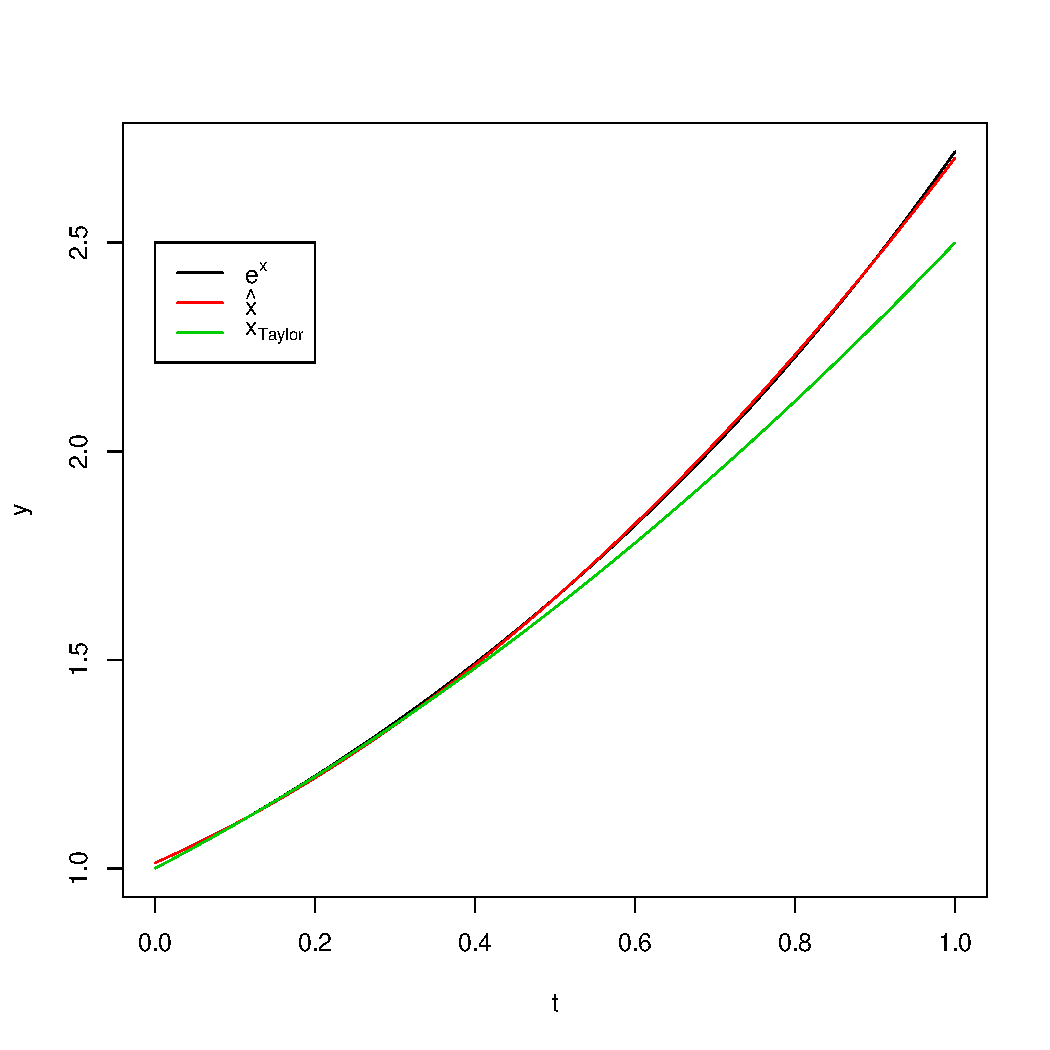
\includegraphics[scale=0.4]{hw1p1.pdf}
\end{center}
\caption{Plot of  $e^t, \hat{x}$ and $x_{Taylor}$. It is clear that  $\hat{x}$ is superior to $x_{Taylor}$.} 
\label{fig:hw1p1}
\end{figure}

Finally, we repeat the exercise with $\norm{x-y} = \int_0^1 16(t-1/2)^2(x(t)-y(t))^2 dt$. Note that
\begin{align*}
&\int_0^1 16(t-1/2)^2(x(t)-y(t))^2 dt \\
&= \int_0^1 16(t-1/2)^2(x(t)^2-2x(t)y(t)-y(t)^2) dt \\
&= \int_0^1 16(t-1/2)^2 x(t)^2 dt -2 \int_0^1 16(t-1/2)^2 x(t)y(t) dt- \int_0^1 16(t-1/2)^2 y(t)^2 dt
\end{align*}
Thus we deduce $<x,y> = \int_0^1 16(t-1/2)^2 x(t)y(t) dt$. In this case, the following $\mathbf{R}$ code solves the required linear system:
\begin{verbatim}
A1 <- matrix(0,nrow = 3, ncol = 3)
A1[1,1] = integrate(function(t){16*(t-1/2)^2*1}, 0, 1)$value
A1[2,1] = A1[1,2] = integrate(function(t){16*(t-1/2)^2*t}, 0, 1)$value
A1[3,1] = A1[1,3] = integrate(function(t){16*(t-1/2)^2*(t^2)}, 0, 1)$value
A1[3,2] = A1[2,3] = integrate(function(t){16*(t-1/2)^2*(t^3)}, 0, 1)$value
A1[2,2] = integrate(function(t){16*(t-1/2)^2*(t^2)}, 0, 1)$value
A1[3,3] = integrate(function(t){16*(t-1/2)^2*(t^4)}, 0, 1)$value

b1 <- matrix(0,nrow = 3, ncol = 1)
b1[1] = integrate(function(t){16*(t-1/2)^2*(exp(t))}, 0, 1)$value
b1[2] = integrate(function(t){16*(t-1/2)^2*(exp(t))*t}, 0, 1)$value
b1[3] = integrate(function(t){16*(t-1/2)^2*(exp(t))*(t^2)}, 0, 1)$value

a1 = solve(A1,b1)
\end{verbatim}

Figure \ref{fig:hw1p1-2} shows how close these two estimates are in predicting $e^t$. In addition, in this case $\norm{x-\hat{x}_1} = 4.42977e^{-05}$, which is virtually the same as the error from $\hat{x}$. Hence, changing the inner product in this case doesn't affect the best linear approximation too much.

\begin{figure}[H]
\begin{center}
  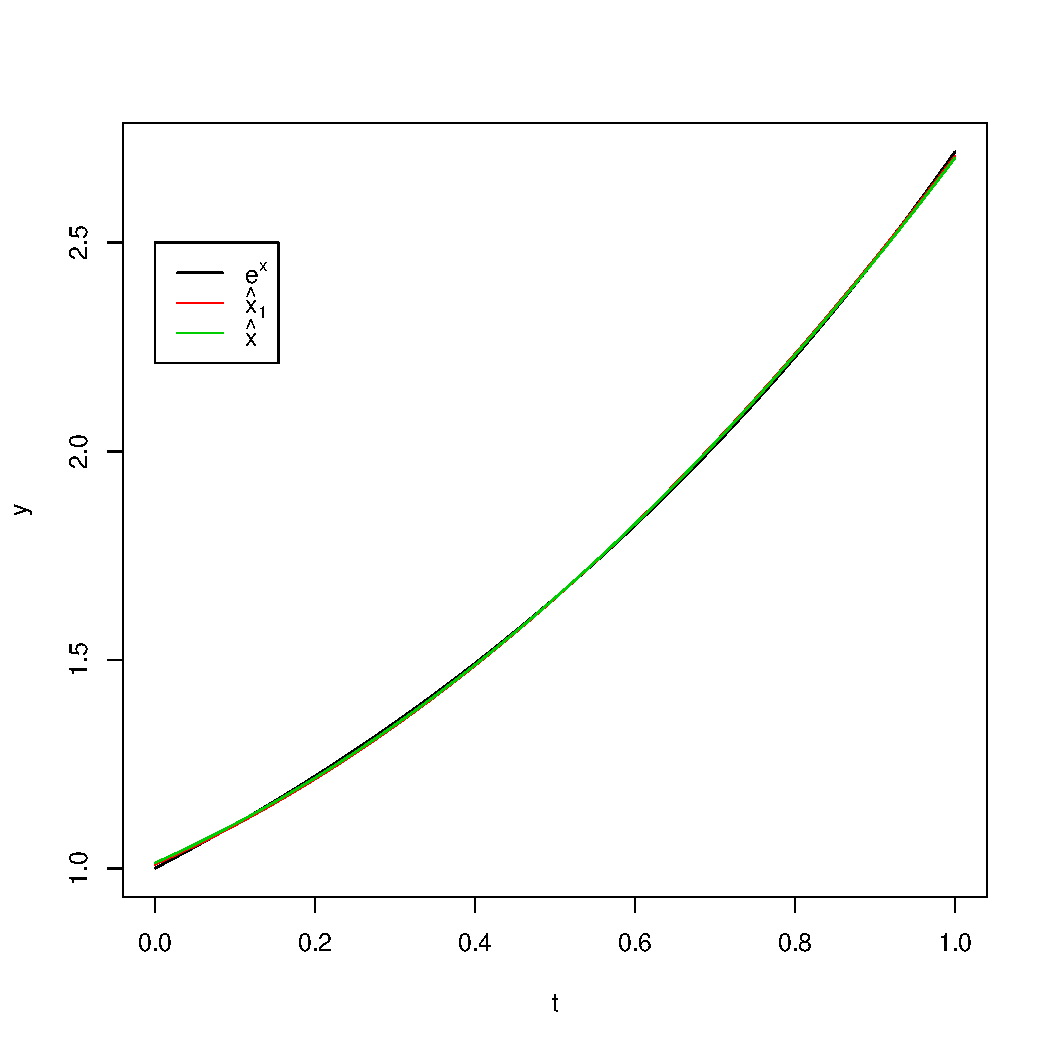
\includegraphics[scale=0.4]{hw1p1-2.pdf}
\end{center}
\caption{Plot of  $e^t, \hat{x}$ and $\hat{x}_1$. Both of them perform about the same.} 
\label{fig:hw1p1-2}
\end{figure}

\paragraph{2}

First note that  
\begin{align*}
&2\int_0^1\cos(\pi n t) \cos(\pi n' t) dt \\
& = \int_0^1 \cos(\pi (n-n') t) + \cos(\pi (n+n') t) dt \\
& = \big[ \frac{\sin(\pi (n-n') t)}{\pi (n-n')} + \frac{\sin(\pi (n+n') t)}{\pi (n+n')} \big]_0^1\\
&= \begin{cases}
1 \text{ if } n=n' \\
0 \text{ if } n\neq n'
\end{cases}
\end{align*}
We can also show that 
$$
\sum_{i = 1}^{N} v_{n}(i)v_{n'}(i) = \begin{cases} 1 \text{ if } n = n' \\
0 \text{ else } \end{cases}
$$ 
Note that $v_0(i)v_0(i) = 1/N \implies \sum_{i = 1}^{N} v_0(i)v_0(i) = 1$. Now note that 
\begin{align*}
\sum_{i = 1}^N v_n(i)v_n(i) &= 2/N \sum_{i = 1}^N \cos^2(\pi n \frac{i-1/2}{N}) \\
&= 2/N (1/4) (\sin(2 \pi n) \csc(\pi n / N) + 2N) \\
&= 1 \\
\end{align*}
Similarly, $\sum_{i = 1}^N v_n(i)v_{n'}(i) = 0$ when $n \neq n'$.

Basically the procedure we would use is to find the orthogonal projection onto the $k-$dimensional subspace spanned by $\mathcal{T}$ where $k$ is a much smaller number than $N$. Doing this in a linear fashion involves finding the best fit coefficients for the first $k$ basis vectors of the space we are interested in and discarding the rest. 

The pictures shown in Figures \ref{fig:fl1},  \ref{fig:fl2} and \ref{fig:tiger} are used for this exercise. The angle between the images in \ref{fig:fl1} and \ref{fig:fl2} 0.546625, while the angle between  \ref{fig:fl2} and \ref{fig:tiger} is 0.7093961 and the angle between \ref{fig:fl1} and \ref{fig:tiger} is 0.6004843. As expected the smallest angle is between the images of the flowers even though it is quite clear that they are very different pictures. 

\begin{figure}
\centering
\subfloat[]
  {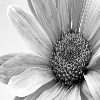
\includegraphics[scale=1]{flower.png}
\label{fig:fl1}}
\subfloat[]
  {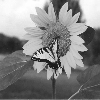
\includegraphics[scale=1]{flower2.png}
\label{fig:fl2}}
\subfloat[]
  {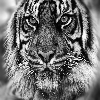
\includegraphics[scale=1]{tiger.png}
\label{fig:tiger}}
\caption{Pictures used for analysis with DCT basis}
\end{figure}

It is simple to show that $$<\phi_{m,n},\phi_{m,n}> = \sum_{i = 1}^N
\sum_{j = 1}^N v_n(i)^2 v_m(j)^2 = \sum_{i = 1}^N  v_n(i)^2 \sum_{j =
  1}^N v_m(j)^2 = 1$$ by the previous part. Using the same part and
the orthogonality of $v_n(i)$ and $v_{n'}(i)$ when $n \neq n'$, we can
show  $$<\phi_{m,n},\phi_{m,n}>  = \sum_{i = 1}^N v_n(i) v_{n'}(i)
\sum_{j = 1}^N  v_m(j) v_{m'}(j) = 0$$, i.e. the 2D DCT basis is
orthogonal. 

\begin{figure}[H]
\begin{center}
  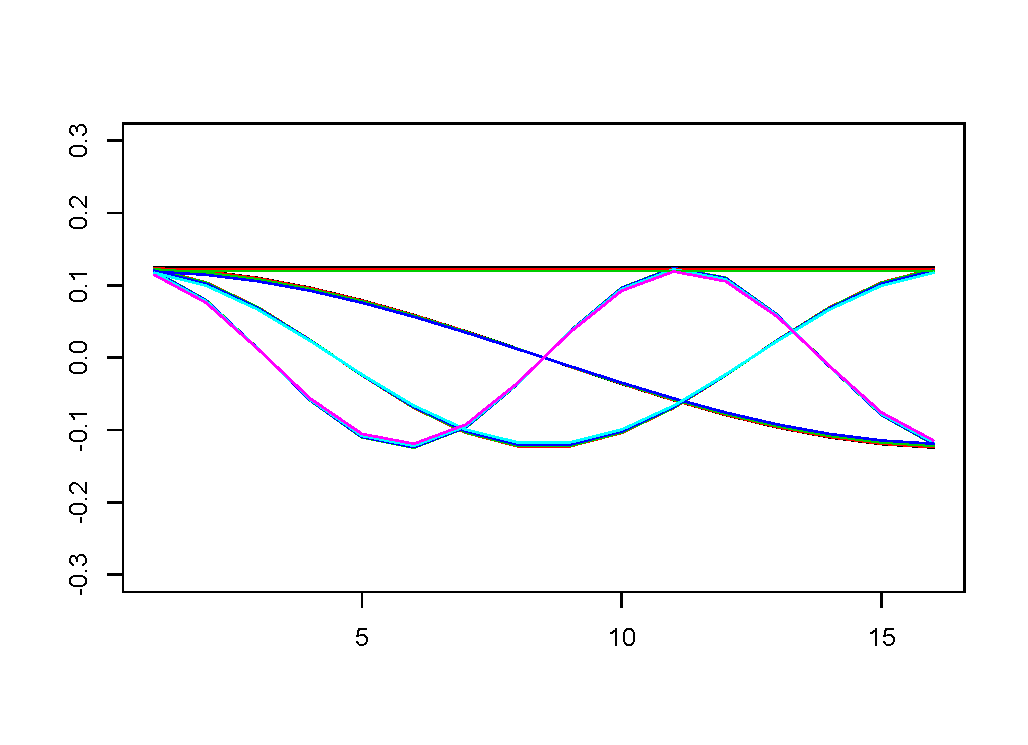
\includegraphics[scale=0.65]{basisplots.pdf}
\end{center}
\caption{Basis Plots} 
\label{fig:basisplots}
\end{figure}

Finally, to construct $\hat{x}_{25\%}$ and for comparing the norm errors versus $k$, the number of basis elements we keep, we use the following $\mathbf{R}$ code as instructed:
\begin{verbatim}
numberk = 10
norm = rep(0,numberk)
k = floor(seq(20,100,length=numberk))
for (kk in 1:numberk){
    Aflower = matrix(0,nrow=k[kk],ncol=k[kk])
    for(n in 1:k[kk]){
        for(m in 1:k[kk]){
            Aflower[m,n] = 
sum(outer(vni(m,1:size,size),vni(n,1:size,size))*flower)
        }
    }

    xhatflower = matrix(0,nrow=size,ncol=size)
    for(n in 1:k[kk]){
        for(m in 1:k[kk]){
            xhatflower = xhatflower + 
Aflower[m,n]*outer(vni(m,1:size,size),vni(n,1:size,size))
        }
    }
    display(channel(xhatflower,"gray"))
    norm[kk] = sqrt(sum((flower - xhatflower)^2))
}
\end{verbatim}
The original images were rediced to $200 \times 200$. As $N = 200$, to get 25\% we only need to go up to $N/2 = 100$. Here we start at very sparse solutions and only go up to $25\%$ as the most densely packed image. It is clear from the plots that $\norm{x - \hat{x}_k}$ decrease as $k$ increases. The image quality also improves. Also as once notices, for some reason, the images became a lot darker upon reconstruction.  

\begin{figure}[H]
\begin{center}
  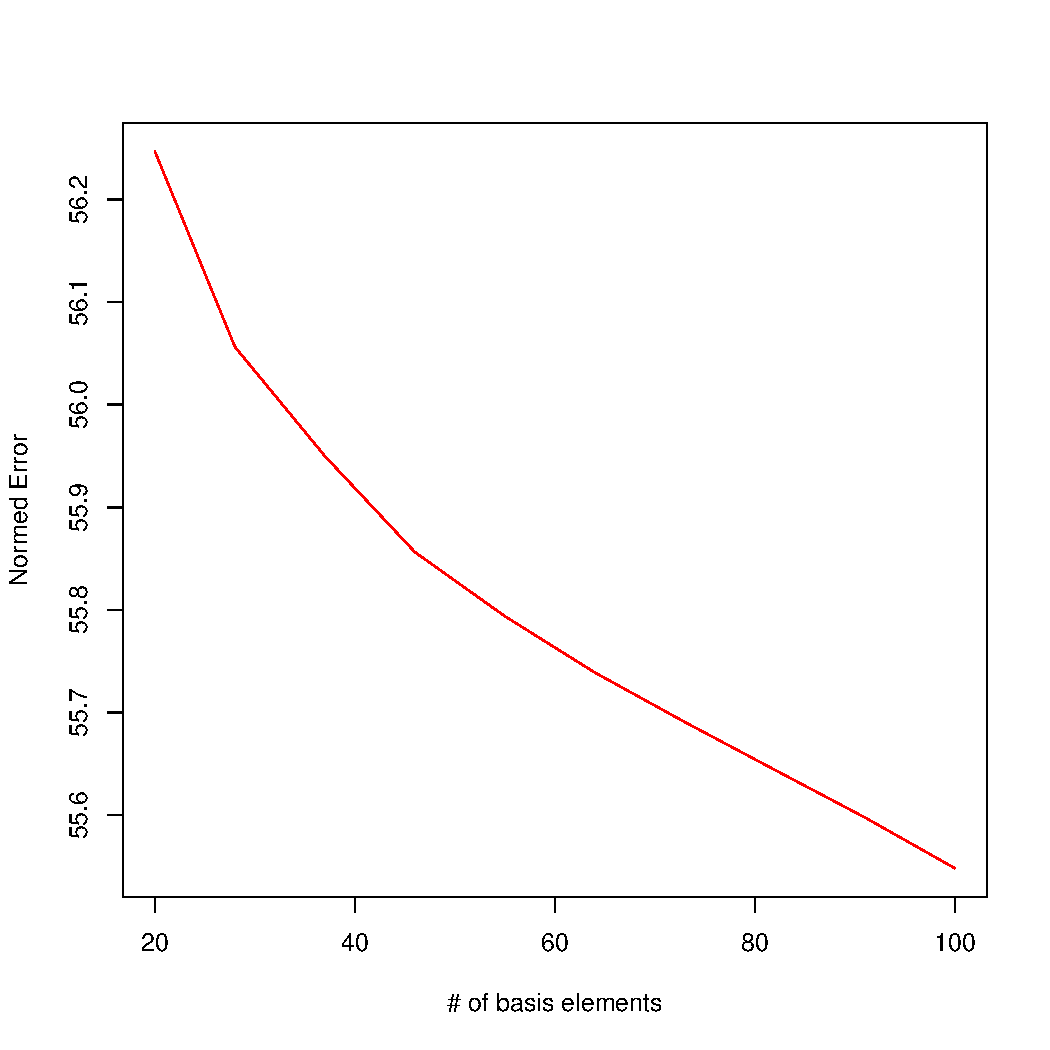
\includegraphics[scale=0.4]{norm2.pdf}
\end{center}
\caption{Plot of Normed Error versus the number of basis elements retained using the DCT} 
\label{fig:hw1p1}
\end{figure}

\begin{figure}
\centering
\subfloat[]
  {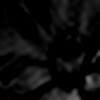
\includegraphics[scale=1]{flk20.png}
\label{fig:flk1}}
\subfloat[]
  {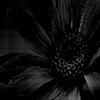
\includegraphics[scale=1]{flk60.png}
\label{fig:flk2}}
\subfloat[]
  {
\includegraphics[scale=1]{flk100.png}
\label{fig:flk2}}
\caption{Pictures reconstucted using DCT basis with k = 10, 55 and 100}
\end{figure}

\end{document}